
\section{2M-TEMPERATURE}
\subsection{DETERMINISTIC EVALUATIONS}

\begin{frame}
\frametitle{DETERMINISTIC EVALUATIONS}
\framesubtitle{Spearman's Rank Correlation}
$$r_s = \frac{\text{cov}(R[H], R[O])}{\sigma_{R[H]} \cdot \sigma_{R[O]}}$$
where:
\begin{itemize}
    \item \( r_s \): Spearman's rank correlation coefficient.
    \item \( H \): Hindcast.
    \item \( O \): Observation.
    \item \( R[x] \): Rank of the variable \( x \).
    \item \( \sigma_x \): Standard deviation of the variable \( x \).
\end{itemize}
\end{frame}

% Frame for Spearman's Rank Correlation Heatmap
\begin{frame}
\frametitle{DETERMINISTIC EVALUATIONS}
\framesubtitle{Spearman's Rank Correlation}
\begin{figure}[H]
    \centering
    \includegraphics[width=1\linewidth]{corr_T2M_ PERIOD.png}
    \caption{Heatmap for Spearman's Rank Correlation (2M Temperature)}
    \label{fig:spearman-correlation}
\end{figure}
\end{frame}

% Frame for RMSE Formula
\begin{frame}
\frametitle{DETERMINISTIC EVALUATIONS}
\framesubtitle{RMSE: Root Mean Square Error}

$$\text{RMSE} = \sqrt{\frac{1}{n} \sum\limits_{i=1}^{n}(H_i - O_i)^2}$$
where:
\begin{itemize}
    \item \( H \): Hindcast.
    \item \( O \): Observation.
    \item \( i \): Index of valid time.
    \item \( n \): Total number of observations.
\end{itemize}
\end{frame}

% Frame for RMSE Heatmap
\begin{frame}
\frametitle{DETERMINISTIC EVALUATIONS}
\framesubtitle{RMSE: Root Mean Square Error}
\begin{figure}[H]
    \centering
    \includegraphics[width=1\linewidth]{rmse_T2M_ PERIOD.png}
    \caption{Heatmap for RMSE (2M Temperature)}
    \label{fig:rmse-heatmap}
\end{figure}
\end{frame}

% Frame for R^2 Formula
\begin{frame}
\frametitle{DETERMINISTIC EVALUATIONS}
\framesubtitle{R-squared (R²)}

\[
R^2 = 1 - \frac{\sum_{i=1}^n (O_i - H_i)^2}{\sum_{i=1}^n (O_i - \bar{O})^2}
\]
where:
\begin{itemize}
    \item \( R^2 \): Coefficient of determination.
    \item \( H_i \): Predicted value (Hindcast).
    \item \( O_i \): Observed value (Observation).
    \item \( \bar{O} \): Mean of observed values.
    \item \( \sum_{i=1}^n (O_i - H_i)^2 \): Residual sum of squares (unexplained variance).
    \item \( \sum_{i=1}^n (O_i - \bar{O})^2 \): Total sum of squares (total variance).
\end{itemize}
\end{frame}

% Frame for R-squared Heatmap
\begin{frame}
\frametitle{DETERMINISTIC EVALUATIONS}
\framesubtitle{R-squared (R²)}
\begin{figure}[H]
    \centering
    \includegraphics[width=1\linewidth]{rsquared_T2M_ PERIOD.png}
    \caption{Heatmap for R² (2M Temperature)}
    \label{fig:rsquared-heatmap}
\end{figure}
\end{frame}


\subsection{Probabilistic Evaluation Metrics}



\begin{frame}
\frametitle{Probabilistic Evaluation Metrics}
\framesubtitle{The Brier Score (BS)}

$$BS_j=\frac{1}{N} \sum\limits_{i}^{N} (y_{j,i} - p_{j,i})^2$$

where:
\begin{itemize}
	\item n is the number of forecasts
	\item $y_{j,i} $ is 1 if the $i^th$ observation was in category $j$, and is 0 otherwise.
	\item $p_{j,i}$  is the $i^th$ forecast probability for category $j$.
\end{itemize}
\end{frame}

\begin{frame}
\frametitle{Probabilistic Evaluation Metrics}
\framesubtitle{The Brier Score (BS)}
\begin{figure}[H]
    \centering
    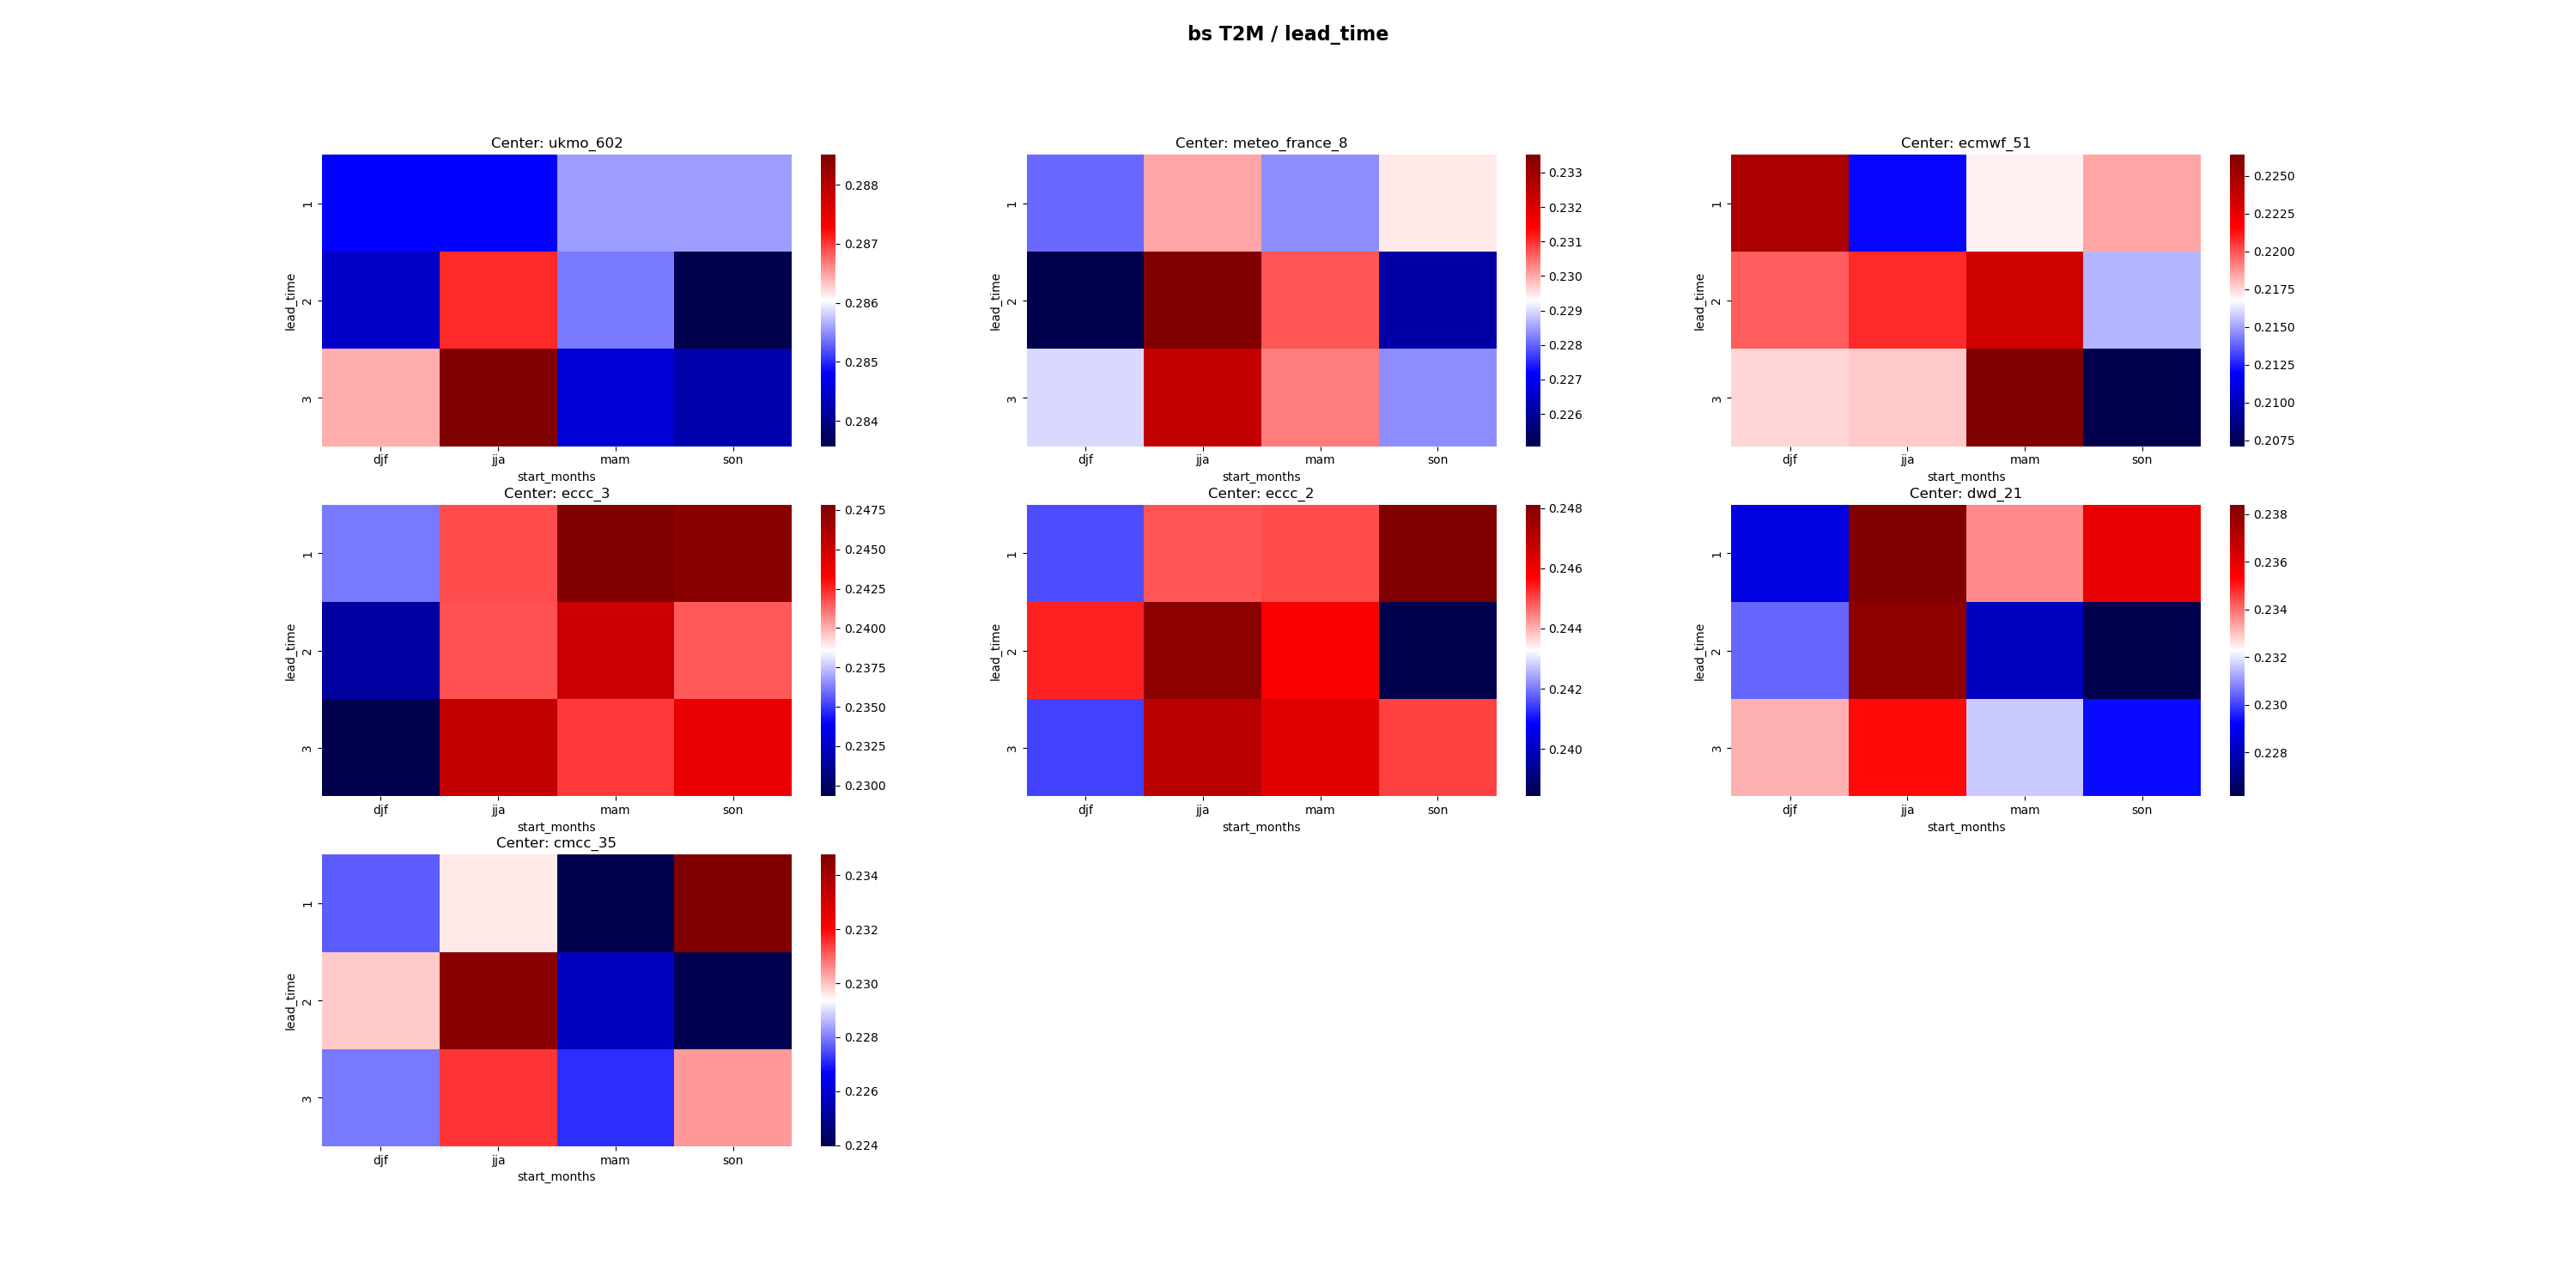
\includegraphics[scale=0.15]{bs_T2M_lead_time.png}
    \caption{The Brier Score for each category  . \textbf{\textit{(0 represents perfect BS)}}}
\end{figure}
\end{frame}




\begin{frame}
\frametitle{Probabilistic Evaluation Metrics}
\framesubtitle{RELIABILITY}

$$Reliability=\frac{1}{n} \sum\limits_{k=1}^{d} n_k(\bar{p_k}-\bar{y_k})^2$$
where:
\begin{itemize}
	\item $n_k$ is the number of forecasts for the $k_th$ probability value ($\bar{p_k}$)
	\item ($\bar{y_k}$) is the observed relative frequency for that value.
\end{itemize} 
\end{frame}




\begin{frame}
\frametitle{Probabilistic Evaluation Metrics}
\framesubtitle{ranked probability score (RPS)}


$$RPS=\frac{1}{n(m-1)}\sum\limits_{i=1}^{n} \sum\limits_{k=1}^{m-1} \left(\sum\limits_{j=1}^{k}(y_{j,i} - p_{j,i})\right)^2  $$

where : 

\begin{itemize}
	\item n is the number of forecasts.
	\item m is the number of categories.
	\item $y_{j,i}$ is 1 if the $i^th$ observation was in category j, and is 0 otherwise.
	\item $p_{j,i}$ is the $i^th$ forecast probability for category j
\end{itemize}
\end{frame}

\begin{frame}
\frametitle{Probabilistic Evaluation Metrics}
\framesubtitle{ranked probability score (RPS)}
\begin{figure}[H]
    \centering
    \includegraphics[scale=0.15]{rps_T2M_ PERIOD.png}
    \caption{The average of  RPS Score on all categories    . \textbf{\textit{(0 means perfect RPS)}}}
\end{figure}
\end{frame}







\begin{frame}
\frametitle{Probabilistic Evaluation Metrics}
\framesubtitle{Relative operating characteristics(ROC)}

\begin{figure}[H]
    \centering
    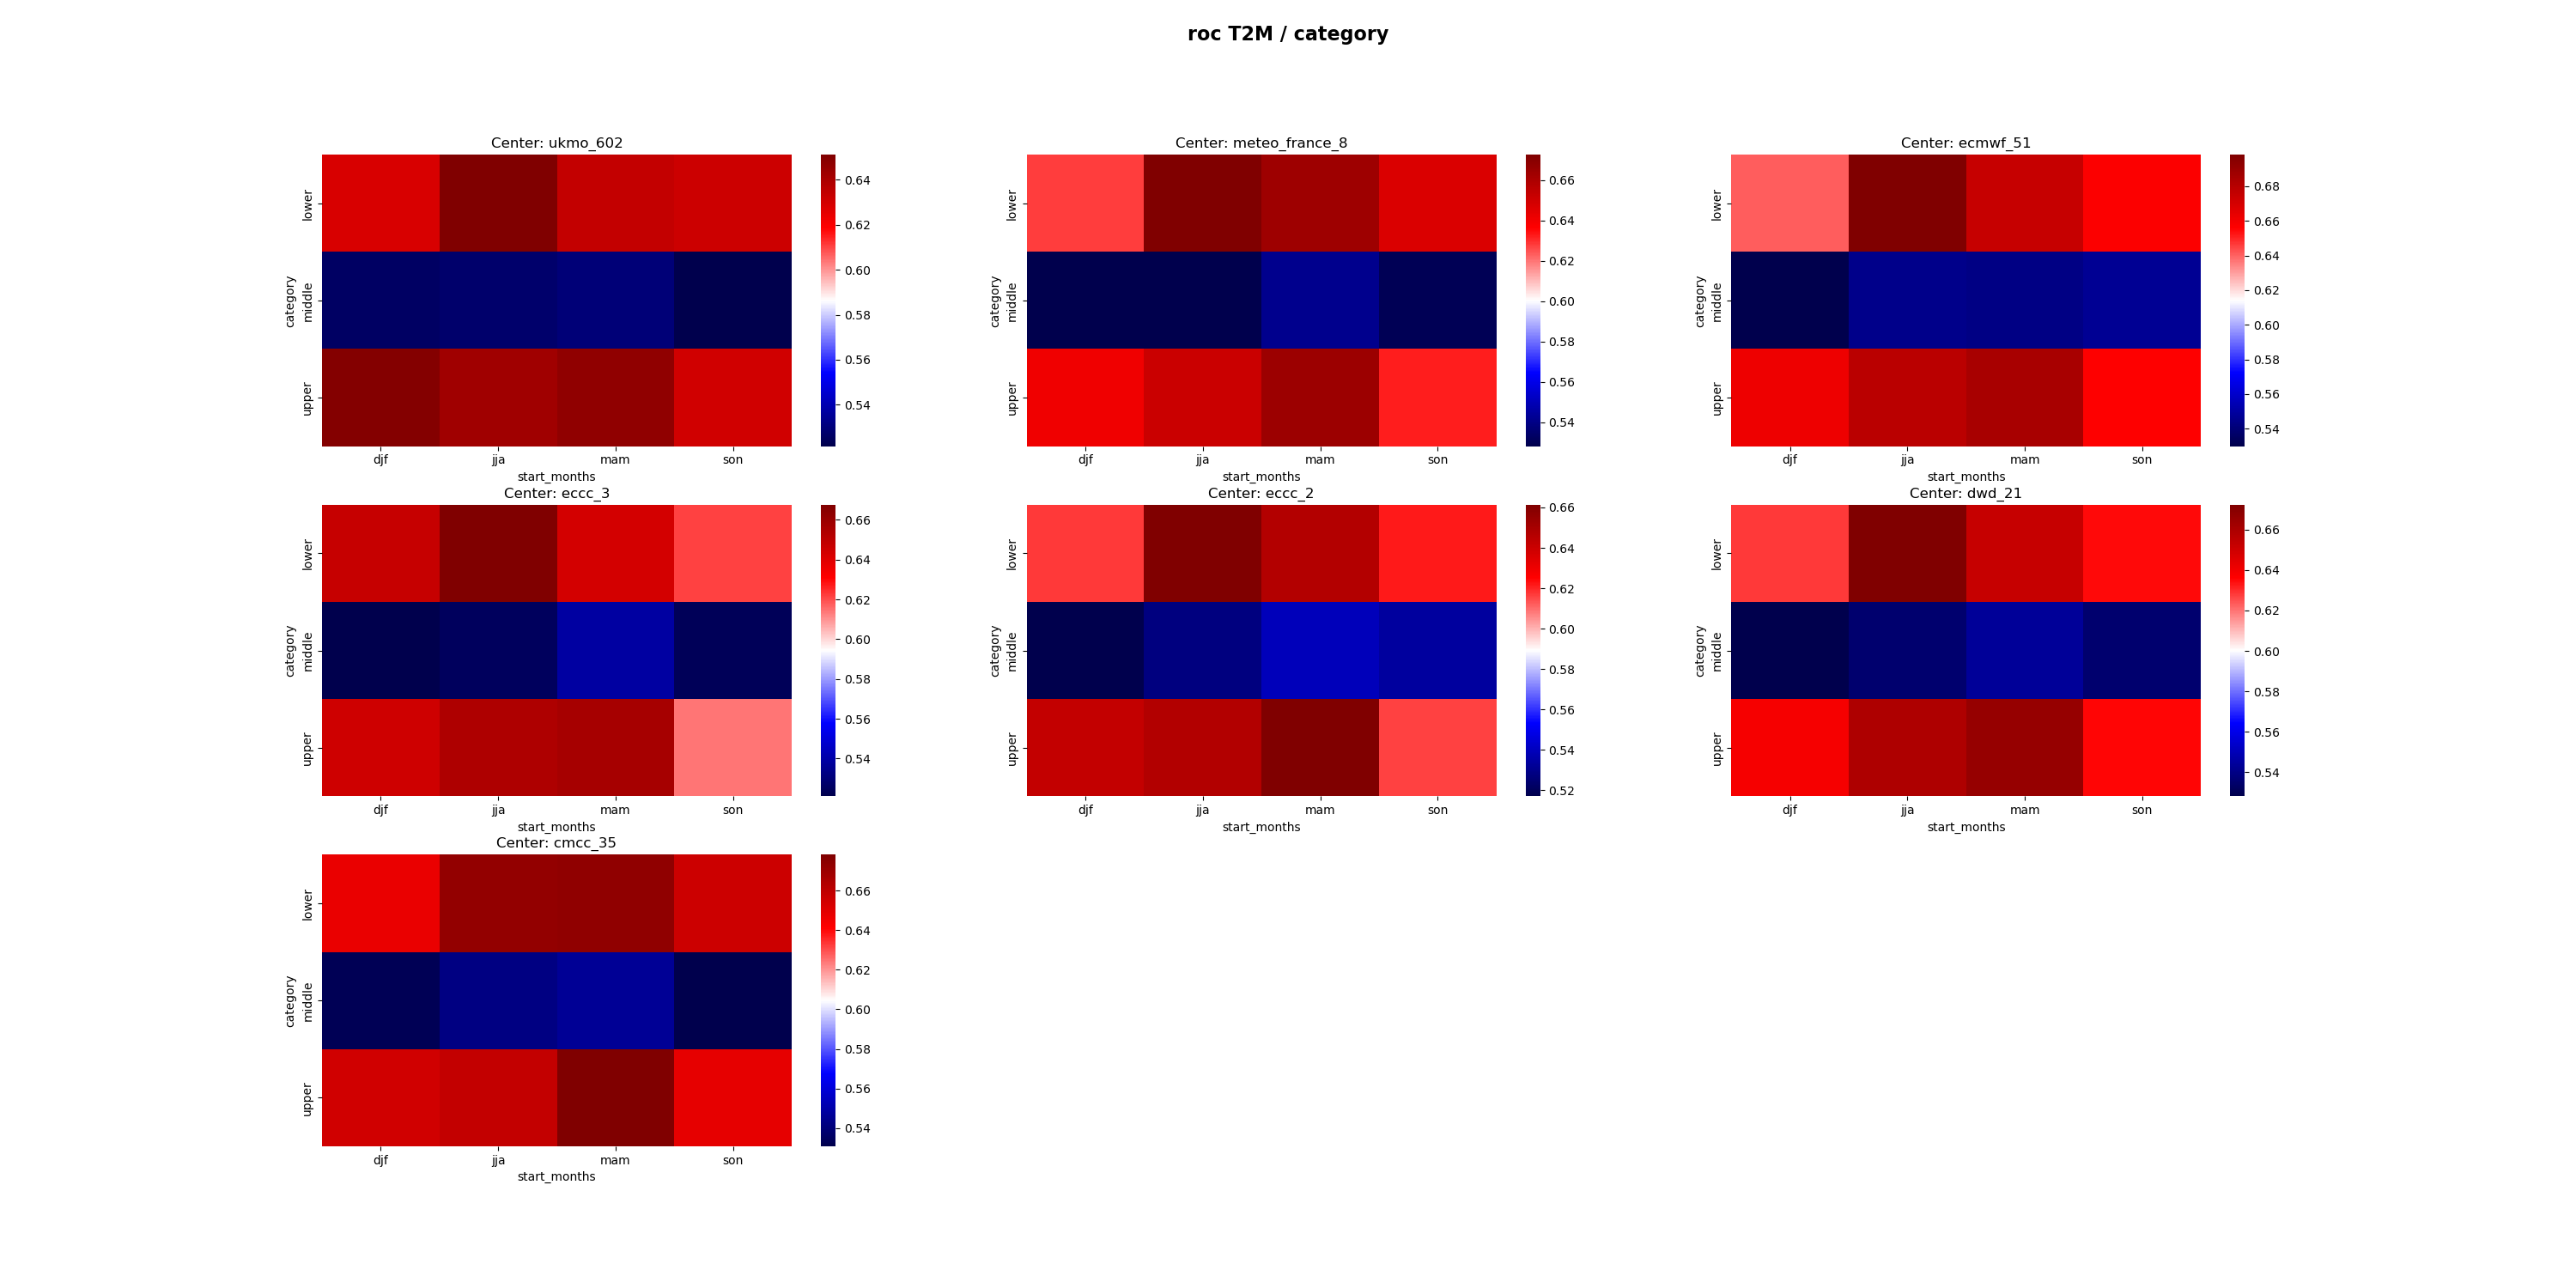
\includegraphics[scale=0.15]{roc_T2M_category.png}
    \caption{The ROC Score for each category  . \textbf{\textit{(1 means perfect ROC)}}}
\end{figure}
\end{frame}

\begin{frame}
\frametitle{Probabilistic Evaluation Metrics}
\framesubtitle{Relative operating characteristics(ROC)}

\begin{figure}[H]
    \centering
    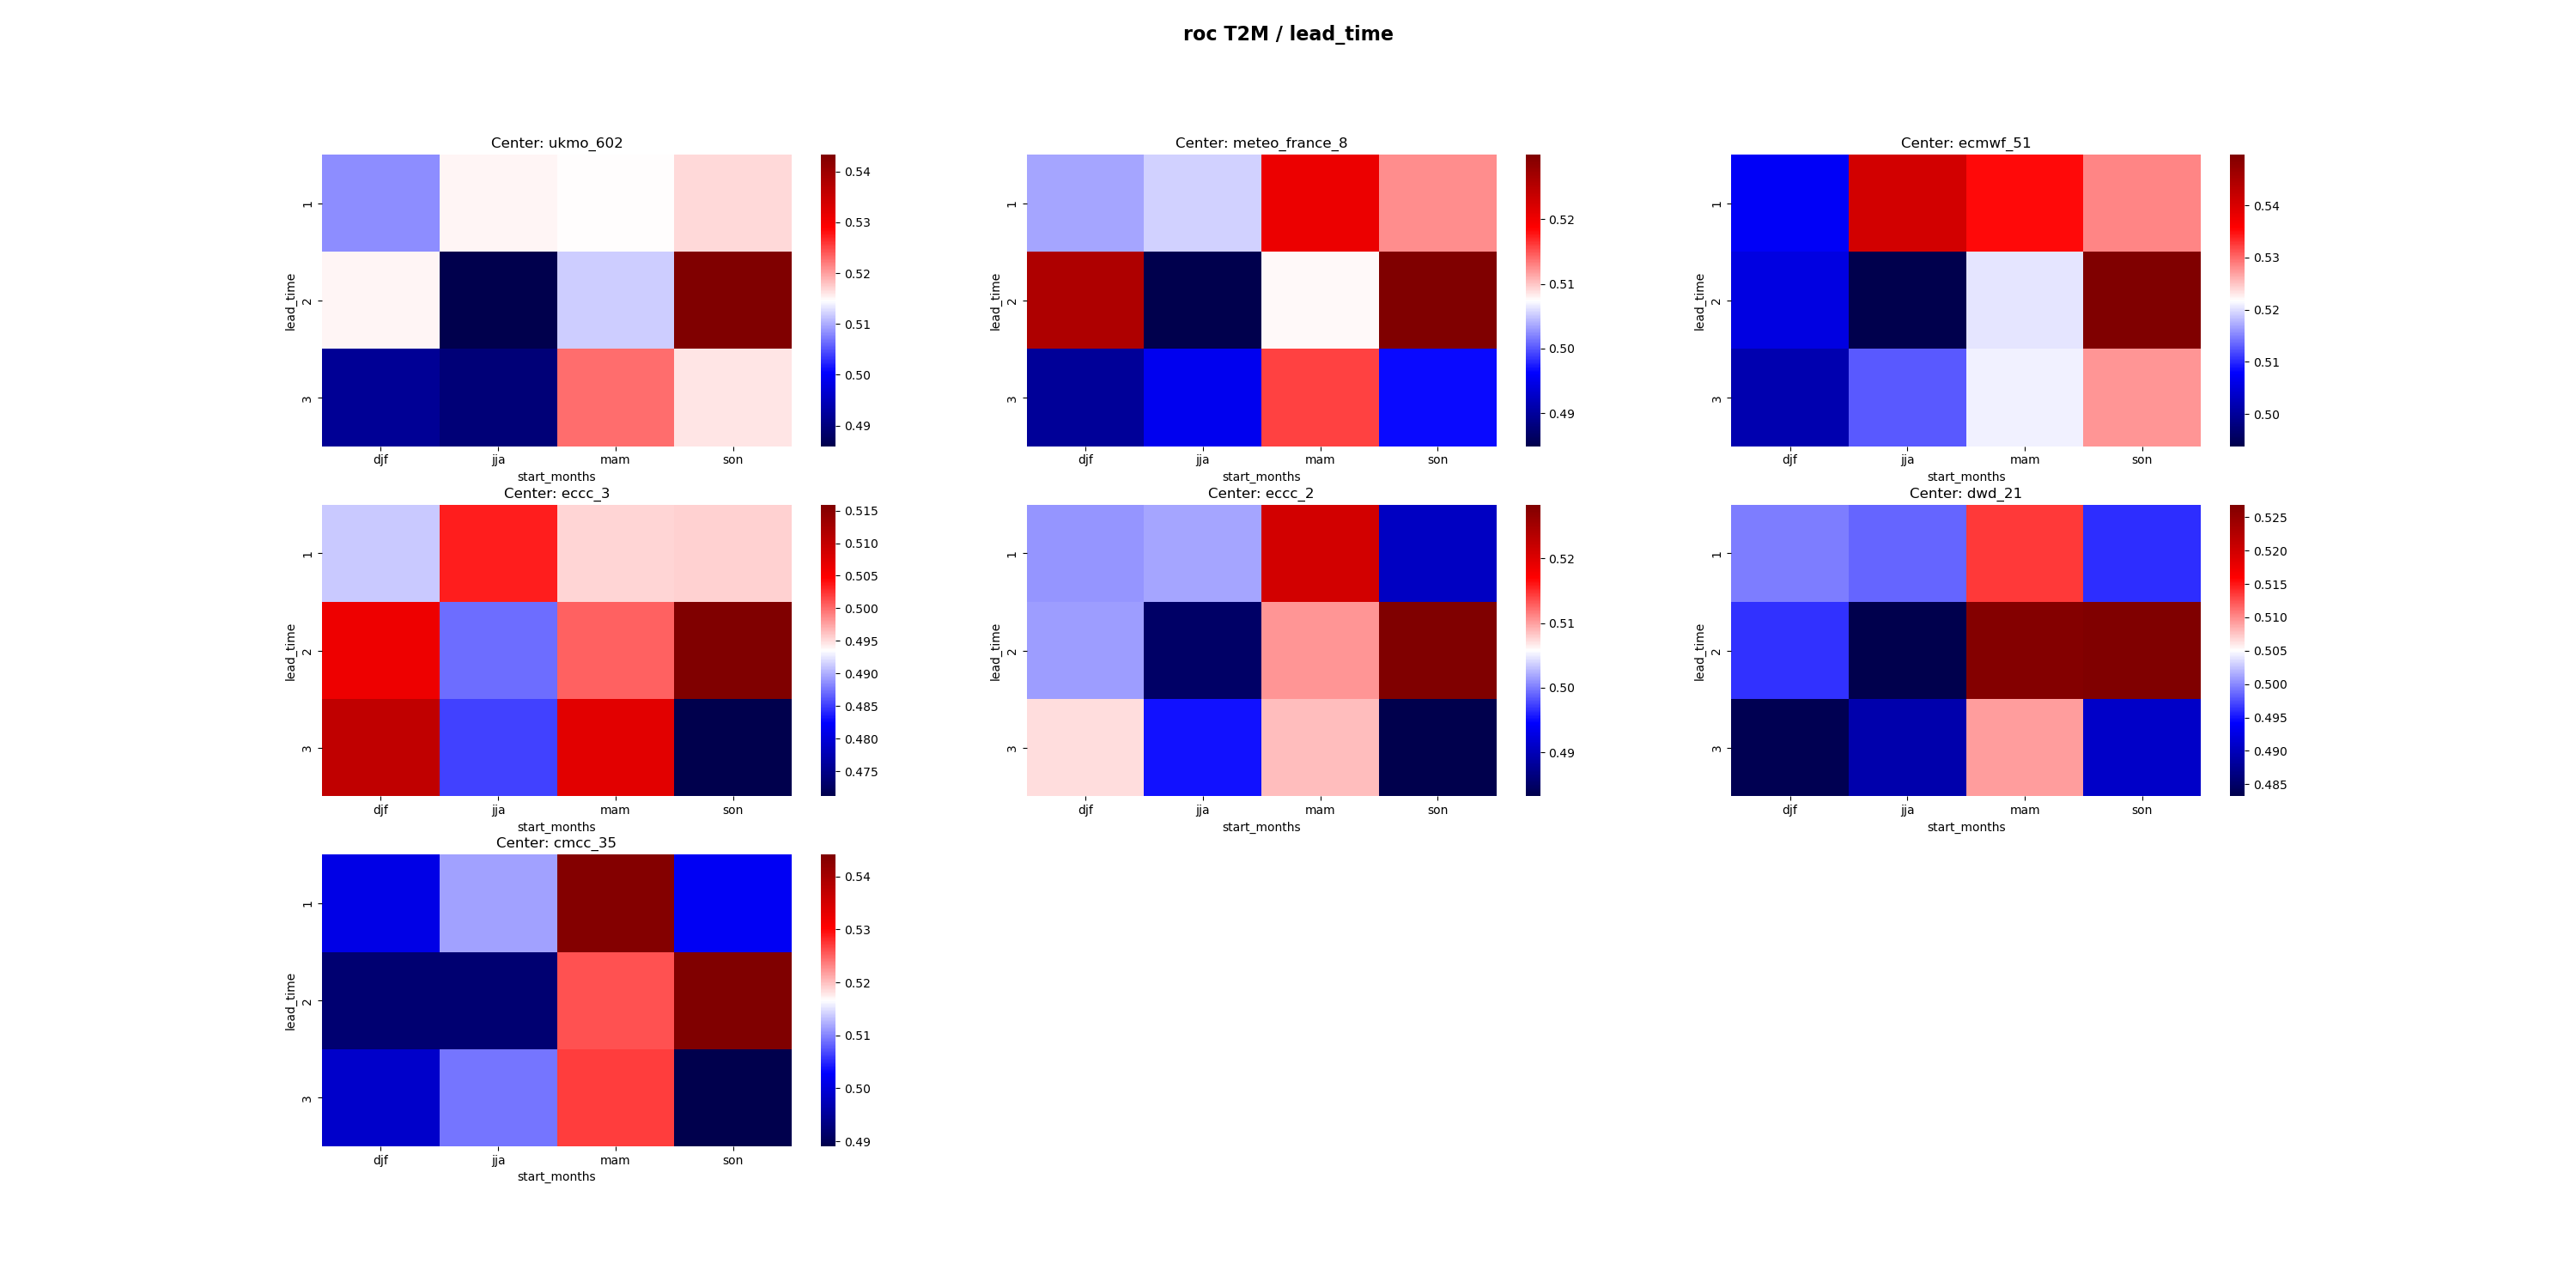
\includegraphics[scale=0.15]{roc_T2M_lead_time.png}
    \caption{The ROC Score for each category  . \textbf{\textit{(1 means perfect ROC)}}}
\end{figure}
\end{frame}


\begin{frame}

\frametitle{Probabilistic Evaluation Metrics}
\framesubtitle{Relative operating characteristics Skill Score(ROCSS)}
	$$ROCSS=\frac{AUC-AUC_{no-skill}}{1-AUC_{no-skill}}$$
where:
\begin{itemize}
	\item $AUC$ : Area Under the ROC Curve for the forecast being evaluated.
	\item $AUC_{no-skill}$ : Area Under the Curve for a no-skill forecast 0.5 for our case.
\end{itemize}

Interpretation of ROCSS:
\begin{itemize}
	\item 1: Perfect discrimination ability.
	\item 0: No skill (forecast performs no better than random guessing).
	\item Negative values: Forecast performs worse than random guessing.
\end{itemize}
\end{frame}


\begin{frame}
\frametitle{Probabilistic Evaluation Metrics}
\framesubtitle{Relative operating characteristics Skill Score(ROCSS)}

\begin{figure}[H]
    \centering
    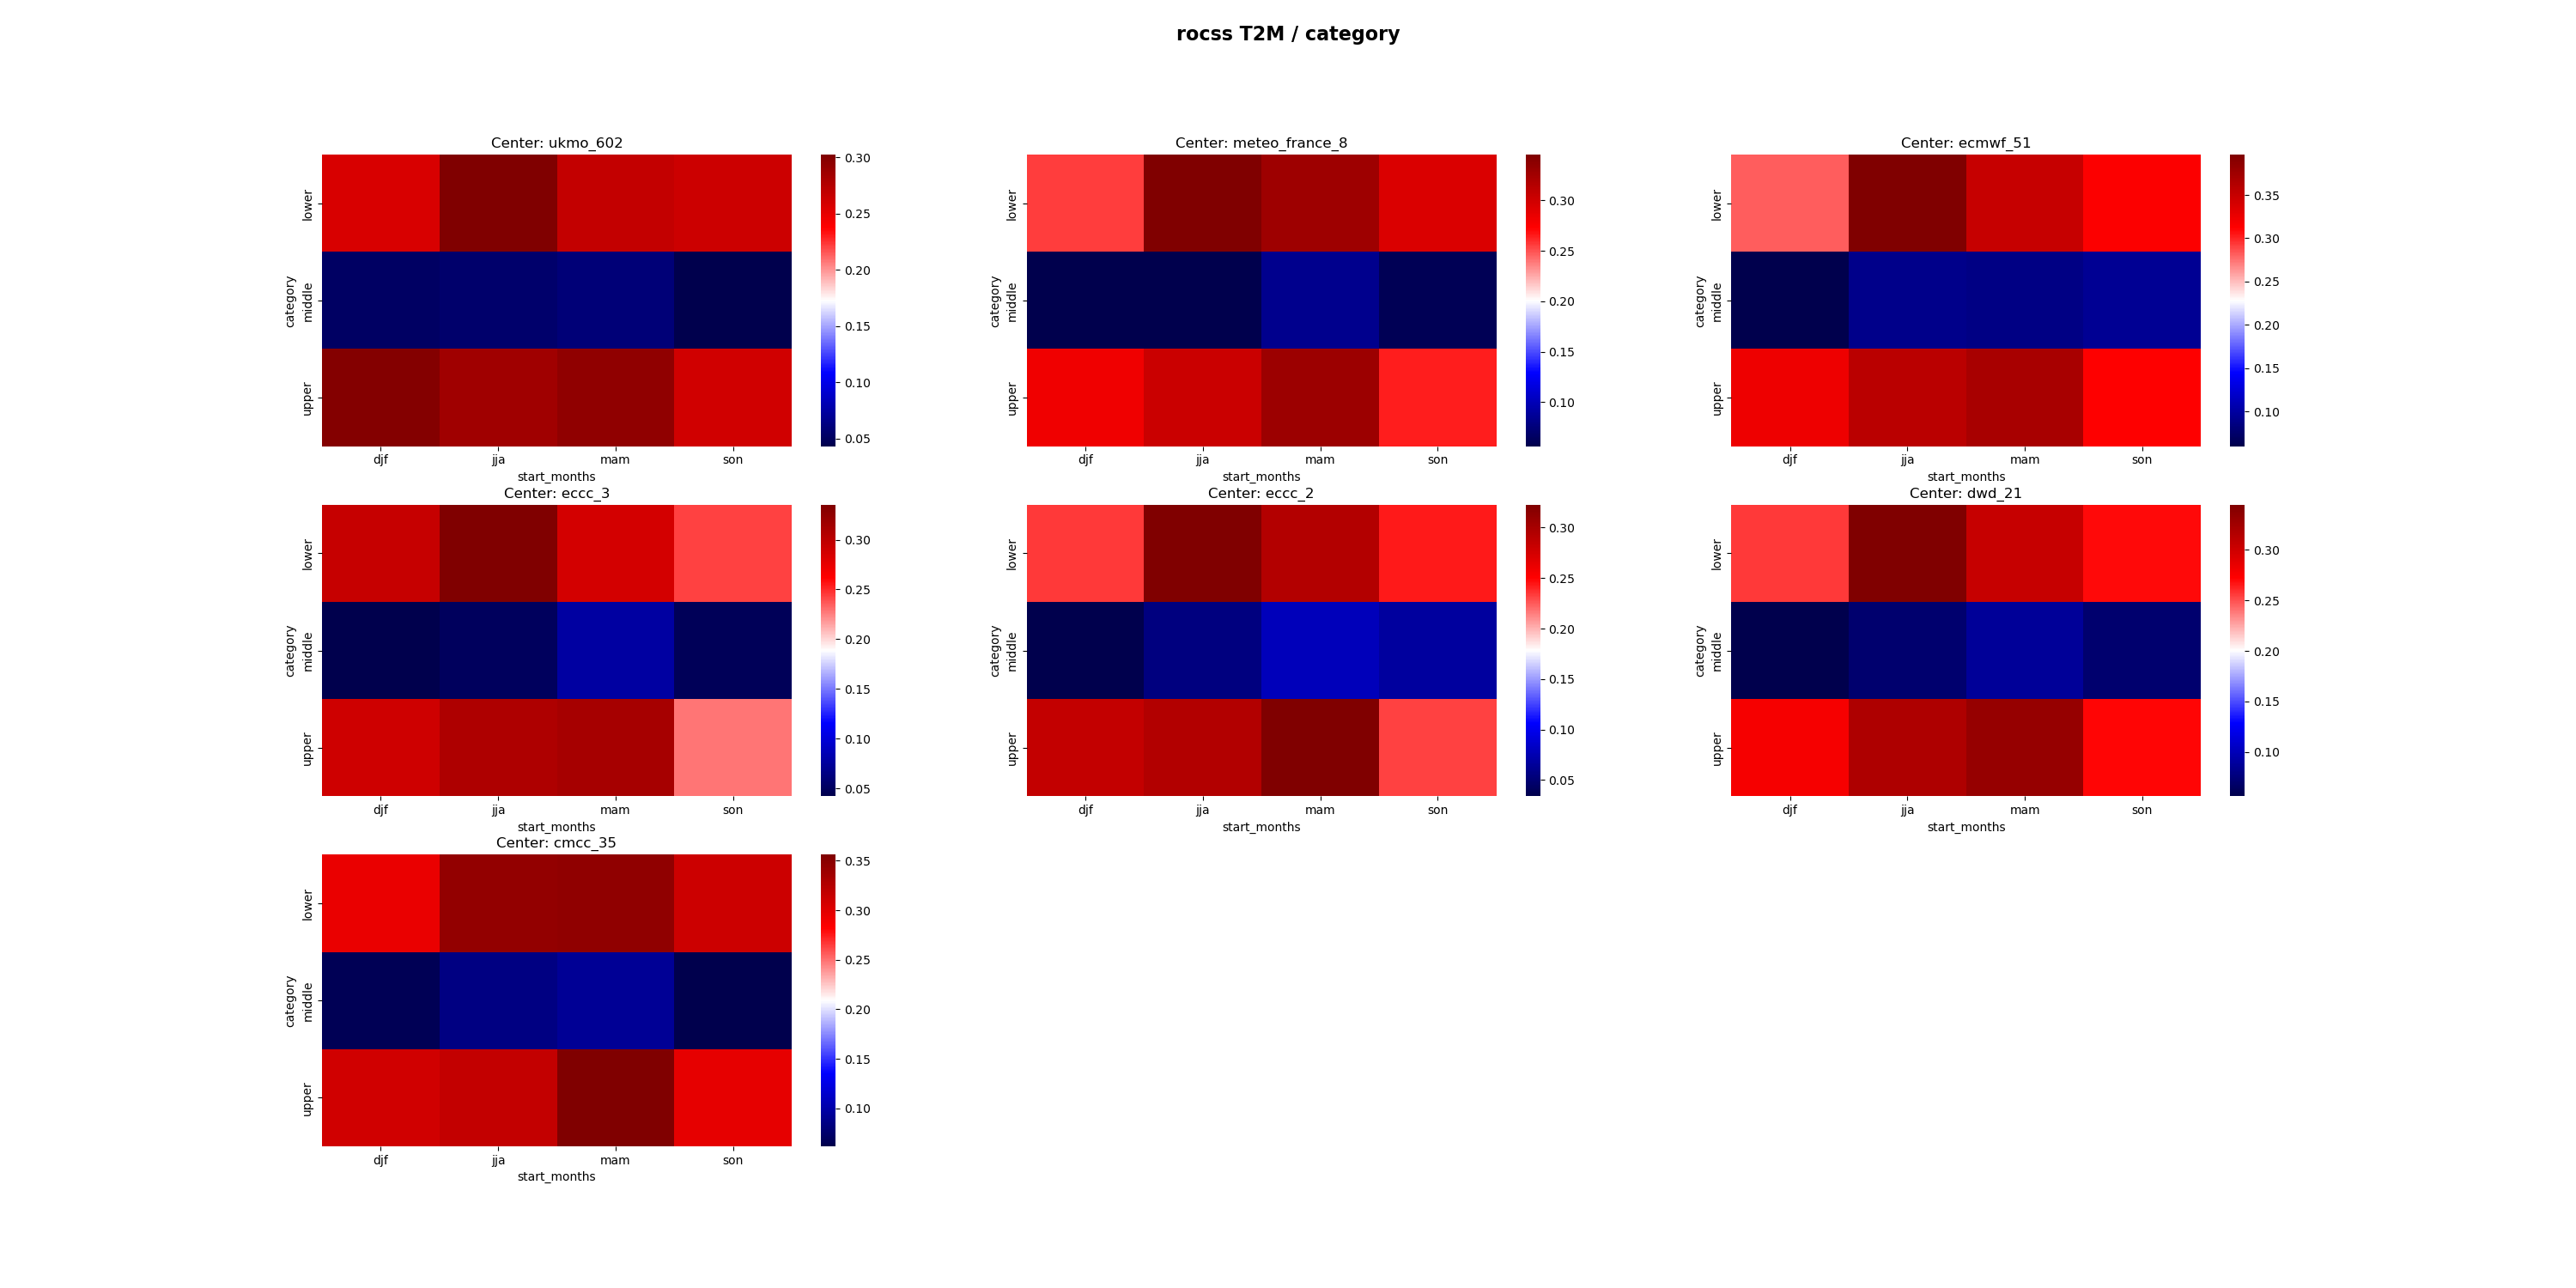
\includegraphics[scale=0.15]{rocss_T2M_category.png}
    \caption{The ROCSS Score for each category  . \textbf{\textit{(1 means perfect ROCSS)}}}
\end{figure}
\end{frame}

\begin{frame}
\frametitle{Probabilistic Evaluation Metrics}
\framesubtitle{Relative operating characteristics Skill Score(ROCSS)}

\begin{figure}[H]
    \centering
    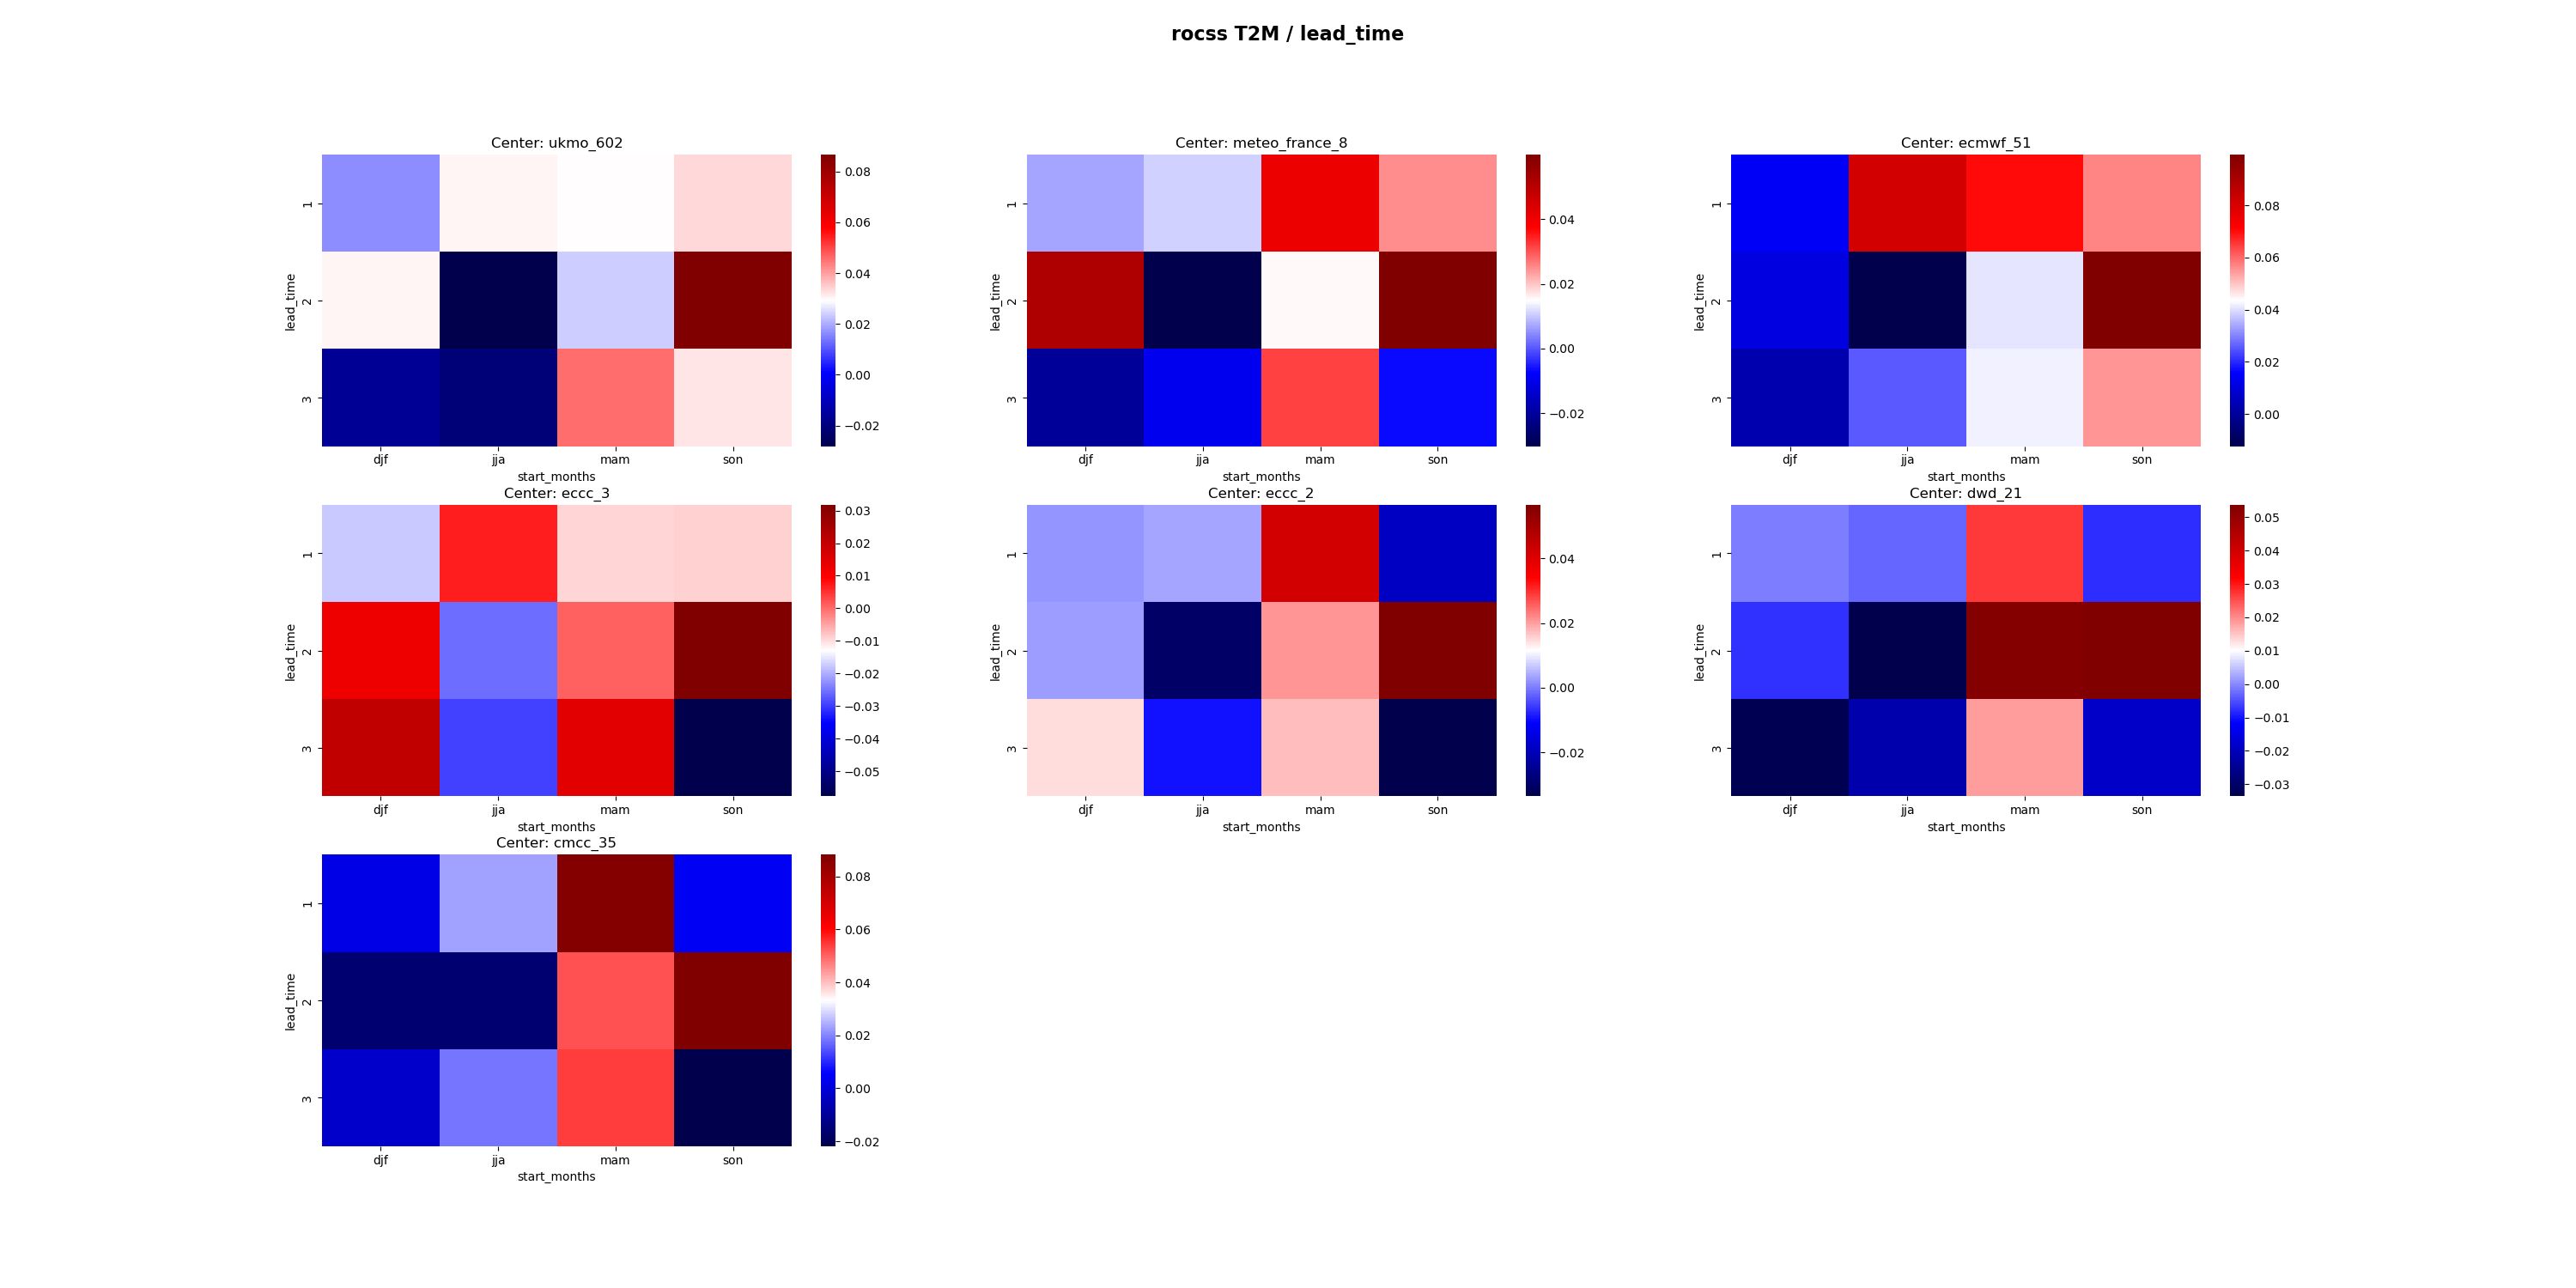
\includegraphics[scale=0.15]{rocss_T2M_lead_time.png}
    \caption{The ROCSS Score for each lead time  . \textbf{\textit{(1 means perfect ROCSS)}}}
\end{figure}
\end{frame}



